\documentclass[11pt]{article}

% ----- preamble -----
\usepackage[a4paper,margin=1.9cm]{geometry}
\usepackage{amsmath,amssymb}
\usepackage{alltt}
\usepackage{tikz}
\usepackage{tikz-cd}
\usetikzlibrary{arrows.meta,positioning,calc,fit,backgrounds,
  shapes.geometric,chains,decorations.pathreplacing}
\usepackage[most]{tcolorbox}
\usepackage{parskip}
\usepackage{xcolor}

\definecolor{ink}{RGB}{40,40,40}
\definecolor{soft}{RGB}{245,245,248}
\definecolor{kas}{RGB}{30,110,190}
\definecolor{grn}{RGB}{30,140,80}

% the three brick colours actually present in the Equation-(1) extract
\definecolor{faceL}{RGB}{30,140,80}   % linearized trace  L
\definecolor{faceF}{RGB}{200,140,0}   % Frobenius / doubling  F
\definecolor{faceC}{RGB}{130,70,170}  % coprime / inverse-mod  C

\newtcolorbox{note}[1][]{colback=soft,colframe=ink,boxrule=0.4pt,
  arc=2pt,left=6pt,right=6pt,top=4pt,bottom=4pt,#1}
\newtcolorbox{leanbox}[1][]{colback=black!4,colframe=black!55,boxrule=0.4pt,
  arc=1.5pt,left=5pt,right=5pt,top=3pt,bottom=3pt,#1}

% code block: alltt keeps ^ _ % $ literal, but \( \) { } still give math/groups
\newenvironment{lean}{\begin{leanbox}\begin{alltt}\small}{\end{alltt}\end{leanbox}}

\tikzset{
  obj/.style={draw=ink,rounded corners=3pt,fill=soft,inner sep=5pt,font=\small,align=center},
  brick/.style={draw=ink,rounded corners=2pt,inner sep=6pt,font=\small,align=center,
    minimum height=13mm},
  thm/.style={draw=ink,rounded corners=3pt,fill=white,inner sep=4pt,
    font=\small,align=center,minimum height=9mm},
  arr/.style={-{Stealth[length=2.5mm]},thick},
  dep/.style={-{Stealth[length=2.4mm]},thick,ink},
  badge/.style={circle,inner sep=0pt,minimum size=3.8mm,font=\scriptsize\bfseries,text=white},
}
\newcommand{\bL}{\tikz[baseline=-0.6ex]\node[badge,fill=faceL]{L};}
\newcommand{\bF}{\tikz[baseline=-0.6ex]\node[badge,fill=faceF]{F};}
\newcommand{\bC}{\tikz[baseline=-0.6ex]\node[badge,fill=faceC]{C};}
\newcommand{\ck}{\textcolor{grn}{\checkmark}}
\newcommand{\lc}[1]{\texttt{\small #1}}

\title{\vspace{-1.5cm}\textbf{The Kasami Equation-(1) LEGO}\\[3pt]
\large Building Dobbertin's Theorem~1, step (1)\,$\Rightarrow$\,(2)\,$\Rightarrow$\,cases,
from the bricks \bL\ and \bF}
\author{\small A picture book of the \texttt{Equation1} Lean formalisation
(Lean\,/\,Mathlib)}
\date{}

\begin{document}
\maketitle
\vspace{-1.0cm}

\begin{note}
\textbf{Scope.} This booklet describes \emph{only} what the \lc{Equation1/}
formalisation actually contains --- the equation-(1) slice of the proof of
Dobbertin's Theorem~1, together with the trace-free Theorem~5 it reuses. It
does \emph{not} cover APN, the MCM bridge (Thm~3/4), the explicit inverse
(Thm~6), Theorem~8, or the difference-set corollaries/conjecture: none of that
material is in this extract. Every box marked \ck\ is \lc{sorry}-free in Lean,
resting only on \lc{propext}, \lc{Classical.choice}, \lc{Quot.sound}.
\end{note}

%======================================================================
\section*{0. The bricks (what is genuinely a building block)}

\begin{center}
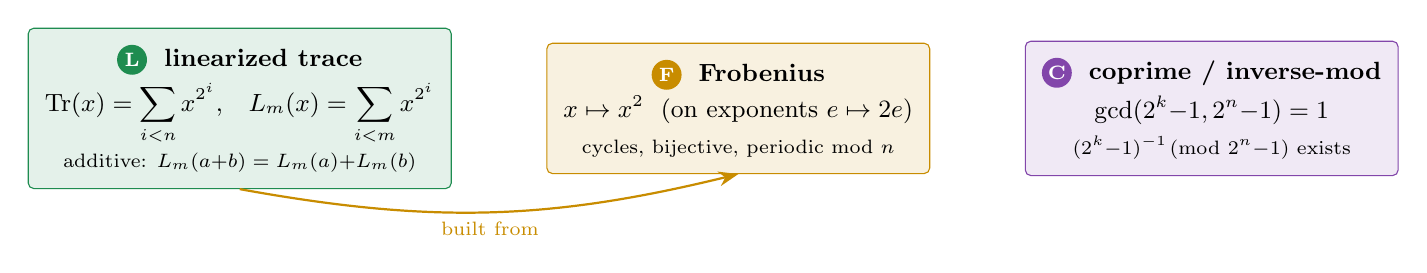
\begin{tikzpicture}[node distance=10mm]
  \node[brick,fill=faceL!12,draw=faceL] (L)
    {\bL\ \ \textbf{linearized trace}\\[2pt]
     $\mathrm{Tr}(x)=\displaystyle\sum_{i<n}x^{2^i}$,\quad
     $L_m(x)=\displaystyle\sum_{i<m}x^{2^i}$\\[2pt]
     \scriptsize additive: $L_m(a{+}b)=L_m(a){+}L_m(b)$};
  \node[brick,fill=faceF!12,draw=faceF,right=12mm of L] (F)
    {\bF\ \ \textbf{Frobenius}\\[2pt]
     $x\mapsto x^{2}$\ \ (on exponents $e\mapsto 2e$)\\[2pt]
     \scriptsize cycles, bijective, periodic mod $n$};
  \node[brick,fill=faceC!12,draw=faceC,right=12mm of F] (C)
    {\bC\ \ \textbf{coprime / inverse-mod}\\[2pt]
     $\gcd(2^k{-}1,2^n{-}1)=1$\\[2pt]
     \scriptsize $(2^k{-}1)^{-1}\!\!\pmod{2^n{-}1}$ exists};
  \draw[arr,faceF] (L.south) to[bend right=12] node[below,font=\scriptsize]{built from} (F.south);
\end{tikzpicture}
\end{center}

\begin{center}\small
The identity that glues \bL\ to \bF\ (Artin--Schreier telescope), \ck:\\[3pt]
$L_m(x)^2+L_m(x)=x^{2^m}+x$\\[2pt]
{\scriptsize(\lc{truncTrace\_sq\_add\_self}, \lc{FiniteFieldPrereqs.lean})}
\end{center}

\medskip
\noindent\textbf{Brick \bL\ --- linearized trace.}
\begin{lean}
def Tr (n : \(\mathbb{N}\)) (x : L) : L := \(\sum\) i \(\in\) range n, x^(2^i)
def truncTrace (m : \(\mathbb{N}\)) (x : F) : F := \(\sum\) i \(\in\) range m, x^(2^i)
lemma truncTrace_add :
    truncTrace m (x + y) = truncTrace m x + truncTrace m y
lemma truncTrace_sq_add_self :
    truncTrace m x ^ 2 + truncTrace m x = x^(2^m) + x
\end{lean}
\emph{Paper.} ``$\mathrm{Tr}$ denotes the trace function from $\mathbb{F}_{2^n}$
onto $\mathbb{F}_2$'' (\S2). The telescope is the mechanism behind
``adding the $2^k$-th power of this equation to itself'' in the proof of Thm~1.

\medskip
\noindent\textbf{Brick \bF\ --- Frobenius / doubling.}
\begin{lean}
lemma frob_cycle (x : F) : x ^ Fintype.card F = x
lemma frob_mod (hn : Fintype.card F = p^n) : x^(p^r) = x^(p^(r % n))
lemma frob_bijective (r : \(\mathbb{N}\)) : Bijective (fun x => x^(p^r))
lemma pow_field_bijective (ha : Coprime (card F - 1) a) :
    Bijective (fun x => x^a)
\end{lean}
\emph{Paper.} the doubling of exponents $2^{ik}$ and the reductions modulo
$2^n-1$ used silently throughout the proof; \lc{pow\_field\_bijective} is what
makes $x\mapsto x^{d}$ a permutation when $\gcd(d,2^n-1)=1$.

\medskip
\noindent\textbf{Brick \bC\ --- coprime / inverse mod $2^n-1$.}
\begin{lean}
theorem mersenne_coprime (h : Coprime k n) :
    Coprime (2^k - 1) (2^n - 1)
theorem inv_mod_exists (h : Coprime k n) (hn : 1 < 2^n - 1) :
    \(\exists\) b, (2^k - 1) * b % (2^n - 1) = 1
\end{lean}
\emph{Paper.} ``First note that $(2^k-1)^{-1}\pmod{2^n-1}$ exists, since
$\gcd(k,n)=1$.'' In this extract \bC\ is present \emph{only} as this
exponent/inverse arithmetic (via $\gcd(2^k{-}1,2^n{-}1)=2^{\gcd(k,n)}-1$), not as
the cyclotomic-coset / difference-set combinatorics of the wider paper.

%======================================================================
\section*{1. The assembled model: definitions built from the bricks}

\begin{center}
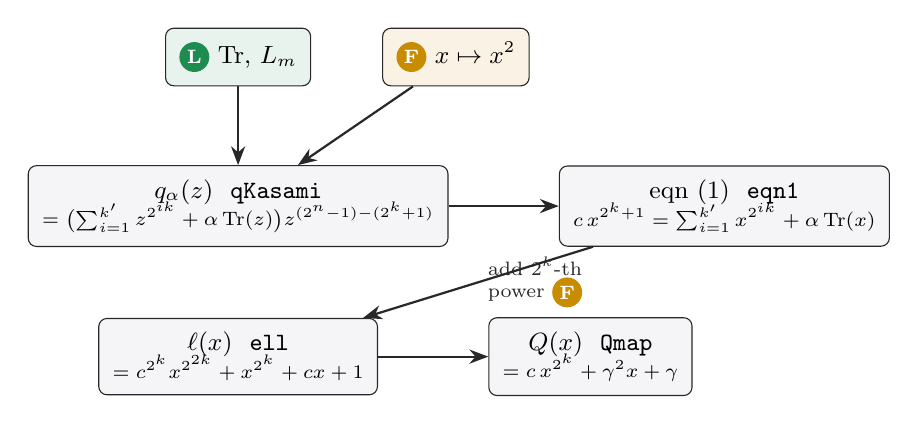
\begin{tikzpicture}[node distance=6mm and 9mm]
  \node[obj,fill=faceL!10] (tr) {\bL\ $\mathrm{Tr}$, $L_m$};
  \node[obj,fill=faceF!10,right=of tr] (fr) {\bF\ $x\mapsto x^2$};
  \node[obj,below=10mm of tr] (q) {$q_\alpha(z)$\ \ \lc{qKasami}\\[-1pt]
     \scriptsize$=\bigl(\sum_{i=1}^{k'}z^{2^{ik}}+\alpha\,\mathrm{Tr}(z)\bigr)z^{(2^n-1)-(2^k+1)}$};
  \node[obj,right=14mm of q] (e1) {eqn (1)\ \ \lc{eqn1}\\[-1pt]
     \scriptsize$c\,x^{2^k+1}=\sum_{i=1}^{k'}x^{2^{ik}}+\alpha\,\mathrm{Tr}(x)$};
  \node[obj,below=9mm of q] (ell) {$\ell(x)$\ \ \lc{ell}\\[-1pt]
     \scriptsize$=c^{2^k}x^{2^{2k}}+x^{2^k}+cx+1$};
  \node[obj,right=14mm of ell] (Q) {$Q(x)$\ \ \lc{Qmap}\\[-1pt]
     \scriptsize$=c\,x^{2^k}+\gamma^2x+\gamma$};
  \draw[dep] (tr) -- (q); \draw[dep] (fr) -- (q);
  \draw[dep] (q) -- (e1);
  \draw[dep] (e1) -- node[right,font=\scriptsize,align=left]{add $2^k$-th\\power \bF} (ell);
  \draw[dep] (ell) -- (Q);
\end{tikzpicture}
\end{center}

\begin{lean}
def qKasami (n k k' \(\alpha\) : \(\mathbb{N}\)) (z : L) : L :=
  ((\(\sum\) i \(\in\) Icc 1 k', z^(2^(i*k))) + (\(\alpha\):L) * Tr n z)
    * z^(2^n - 1 - (2^k+1))
def eqn1 (n k k' \(\alpha\) : \(\mathbb{N}\)) (c x : L) : Prop :=
  c * x^(2^k+1) = (\(\sum\) i \(\in\) Icc 1 k', x^(2^(i*k))) + (\(\alpha\):L) * Tr n x
def ell  (k : \(\mathbb{N}\)) (c x : L) : L := c^(2^k)*x^(2^(2*k)) + x^(2^k) + c*x + 1
def ell0 (k : \(\mathbb{N}\)) (c x : L) : L := ell k c x + 1
def Qmap (k : \(\mathbb{N}\)) (c \(\gamma\) x : L) : L := c*x^(2^k) + \(\gamma\)^2*x + \(\gamma\)
\end{lean}

\emph{Paper.} $q_\alpha$ is the ``generalized Kasami polynomial'' of \S2 (with
$1/z^{2^k+1}$ realised as $z^{(2^n-1)-(2^k+1)}$, convention $0/0=0$); \lc{eqn1}
is equation~(1); \lc{ell} is $\ell(x)$ of equation~(2); \lc{ell0} its
homogeneous part $\ell_0=\ell+1$; \lc{Qmap} is $Q(x)=cx^{2^k}+\gamma^2x+\gamma$
of Case~2.

%======================================================================
\section*{2. Snapping the bricks together: (1) $\Rightarrow$ (2) $\Rightarrow$ cases $\Rightarrow$ Thm 1}

\begin{center}
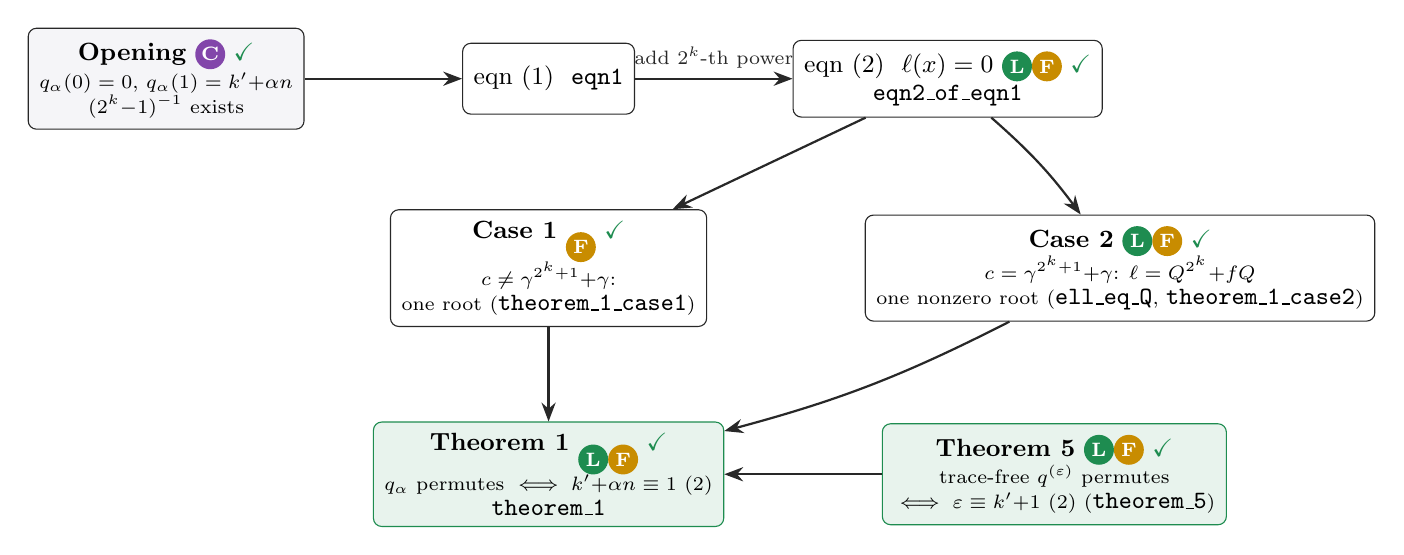
\begin{tikzpicture}[node distance=7mm and 20mm]
  \node[thm,fill=soft] (open)
    {\textbf{Opening} \bC\ \ck\\[-1pt]
     \scriptsize$q_\alpha(0)=0$,\ $q_\alpha(1)=k'{+}\alpha n$\\[-2pt]
     \scriptsize $(2^k{-}1)^{-1}$ exists};
  \node[thm,right=of open] (e1) {eqn (1)\ \ \lc{eqn1}};
  \node[thm,right=of e1] (e2)
    {eqn (2)\ \ $\ell(x)=0$ \bL\bF\ \ck\\[-1pt]
     \scriptsize \lc{eqn2\_of\_eqn1}};
  \node[thm,below=12mm of e1] (c1)
    {\textbf{Case 1} \bF\ \ck\\[-1pt]
     \scriptsize $c\neq\gamma^{2^k+1}{+}\gamma$:\\[-2pt]
     \scriptsize one root (\lc{theorem\_1\_case1})};
  \node[thm,right=of c1] (c2)
    {\textbf{Case 2} \bL\bF\ \ck\\[-1pt]
     \scriptsize $c=\gamma^{2^k+1}{+}\gamma$: $\ell=Q^{2^k}{+}fQ$\\[-2pt]
     \scriptsize one nonzero root (\lc{ell\_eq\_Q}, \lc{theorem\_1\_case2})};
  \node[thm,below=12mm of c1,fill=grn!10,draw=grn] (t1)
    {\textbf{Theorem 1} \bL\bF\ \ck\\[-1pt]
     \scriptsize $q_\alpha$ permutes $\iff k'{+}\alpha n\equiv1\ (2)$\\[-2pt]
     \scriptsize \lc{theorem\_1}};
  \node[thm,right=of t1,fill=grn!10,draw=grn] (t5)
    {\textbf{Theorem 5} \bL\bF\ \ck\\[-1pt]
     \scriptsize trace-free $q^{(\varepsilon)}$ permutes\\[-2pt]
     \scriptsize $\iff\varepsilon\equiv k'{+}1\ (2)$ (\lc{theorem\_5})};

  \draw[dep] (open) -- (e1);
  \draw[dep] (e1) -- node[above,font=\scriptsize]{add $2^k$-th power} (e2);
  \draw[dep] (e2) -- (c1);
  \draw[dep] (e2) to[bend left=6] (c2);
  \draw[dep] (c1) -- (t1);
  \draw[dep] (c2) to[bend left=6] (t1);
  \draw[dep] (t5) -- (t1);
\end{tikzpicture}
\end{center}

\begin{center}\small
\bL\ linearized trace \quad \bF\ Frobenius \quad \bC\ coprime/inverse-mod
\qquad \ck\ \lc{sorry}-free in Lean
\end{center}

%----------------------------------------------------------------------
\subsection*{2.0 Opening (before equations (1)/(2))}
\begin{lean}
theorem qKasami_zero : qKasami n k k' \(\alpha\) 0 = 0
theorem Tr_one : Tr n (1 : L) = (n : L)
theorem qKasami_one : qKasami n k k' \(\alpha\) 1 = ((k' + \(\alpha\)*n : \(\mathbb{N}\)) : L)
theorem qKasami_one_eq_zero_iff :
    qKasami n k k' \(\alpha\) 1 = 0 \(\leftrightarrow\) (k' + \(\alpha\)*n) % 2 = 0
\end{lean}
\emph{Paper.} ``We have $q_\alpha(0)=0$, using the convention `$0/0=0$'. To
verify the `only if' part, observe that $k'+\alpha n\equiv0\pmod 2$ is equivalent
to $q_\alpha(1)=k'\cdot1+\alpha\cdot\mathrm{Tr}(1)=0$.'' (Uses brick \bC\ for the
inverse and brick \bL\ to evaluate $\mathrm{Tr}(1)=n$.)

%----------------------------------------------------------------------
\subsection*{2.1 The step (1) $\Rightarrow$ (2): the telescope in action}
\begin{lean}
theorem eqn2_of_eqn1 (hn : Fintype.card L = 2^n) (hkk1 : k*k' % n = 1)
    (\(\alpha\) : \(\mathbb{N}\)) (c x : L) (hx : x \(\neq\) 0) (h : eqn1 n k k' \(\alpha\) c x) :
    ell k c x = 0
\end{lean}
\emph{Paper.} ``Adding the $2^k$-th power of this equation to itself we get
$\dots$ and consequently $\ell(x)=c^{2^k}x^{2^{2k}}+x^{2^k}+cx+1=0$'' --
equation~(2). This is exactly \bF\ (raise to $2^k$, i.e.\ apply Frobenius $k$
times) fed into \bL\ (the additive telescope \lc{truncTrace\_sq\_add\_self}).\\[2pt]
\emph{Correction (documented in the file).} The bare skeleton is false at
$x=0$: \lc{eqn1} holds vacuously there ($0=0$) while $\ell(0)=1\neq0$. The
faithful statement adds $x\neq0$ and the field hypotheses.

%----------------------------------------------------------------------
\subsection*{2.2 Case 1 --- $c$ not of the form $\gamma^{2^k+1}+\gamma$}
\begin{lean}
theorem theorem_1_case1 (hn : Fintype.card L = 2^n) (hk0 : 0 < k) (hkn : k < n)
    (c : L) (hc : \(\forall\) \(\gamma\) : L, c \(\neq\) \(\gamma\)^(2^k+1) + \(\gamma\)) :
    \{x : L | ell k c x = 0\}.ncard = 1
\end{lean}
\emph{Paper.} ``the homogeneous part $\ell_0(x)=\ell(x)+1$ of (2) has no
non-zero solution $\dots$ Hence (2) has precisely one solution, and we are
done.'' The Lean proof makes the linear map
$\varphi(x)=c^{2^k}x^{2^{2k}}+x^{2^k}+cx$ injective (additivity is brick
\bL/\bF), hence bijective on a finite field, so $\varphi(x)=1$ has a unique
solution.

%----------------------------------------------------------------------
\subsection*{2.3 Case 2 --- $c=\gamma^{2^k+1}+\gamma$}
\begin{lean}
theorem ell_eq_Q (k : \(\mathbb{N}\)) (c \(\gamma\) x : L) (h\(\gamma\) : \(\gamma\) \(\neq\) 0)
    (hc : c = \(\gamma\)^(2^k+1) + \(\gamma\)) :
    ell k c x = Qmap k c \(\gamma\) x ^ (2^k)
      + (\(\gamma\)^(2^k-1) + \(\gamma\)\(^{-1}\)) * Qmap k c \(\gamma\) x
theorem theorem_1_case2 (hn : Fintype.card L = 2^n) \(\dots\) (hc0 : c \(\neq\) 0)
    (hc : c = \(\gamma\)^(2^k+1) + \(\gamma\)) :
    \{x : L | x \(\neq\) 0 \(\wedge\) eqn1 n k k' \(\alpha\) c x\}.ncard = 1
\end{lean}
\emph{Paper.} ``Setting $Q(x)=cx^{2^k}+\gamma^2x+\gamma$,
$f=\gamma^{2^k-1}+1/\gamma$ we have $\ell(x)=Q(x)^{2^k}+fQ(x)$ $\dots$ precisely
one of the solutions $\dots$ is a solution of (1).''\\[2pt]
\emph{Correction (documented in the file).} $x=0$ always satisfies the cleared
\lc{eqn1}, so the faithful count is of \emph{nonzero} solutions (needs $c\neq0$).

%----------------------------------------------------------------------
\subsection*{2.4 The headline: Theorem 1 (and its trace-free twin, Theorem 5)}
\begin{lean}
theorem theorem_1 (hn : Fintype.card L = 2^n) (hk : k < n) (hcop : Coprime k n)
    (hk' : k*k' % n = 1 % n) (hk0 : 0 < k) (hexp : 2^k+1 < 2^n-1)
    (\(\alpha\) : \(\mathbb{N}\)) (h\(\alpha\) : \(\alpha\) = 0 \(\vee\) \(\alpha\) = 1) :
    Bijective (qKasami n k k' \(\alpha\)) \(\leftrightarrow\) (k' + \(\alpha\)*n) % 2 = 1
theorem theorem_5 \(\dots\) :
    Bijective (qeps n k k' \(\varepsilon\)) \(\leftrightarrow\) (\(\varepsilon \equiv\) k'+1  (mod 2))
\end{lean}
\emph{Paper.} ``Theorem~1. A generalized Kasami polynomial $q_\alpha$ is a
permutation polynomial on $L$ iff $k'+\alpha n\equiv1\pmod2$.'' and
``Theorem~5. $q^{(\varepsilon)}$ is a permutation polynomial on $L$ iff
$\varepsilon\equiv k'+1\pmod2$. Again the proof of Theorem~1 can be applied.''
The Lean \lc{theorem\_1} routes $\alpha=0$ through \lc{theorem\_5} and
$\alpha=1$ through the trace-general \lc{gmap\_bijective\_iff}.

%======================================================================
\section*{3. Supporting bricks actually used (Theorem 5 / trace layer)}

These are the intermediate parts, all in the extract, that the assembly above
leans on --- still nothing but \bL, \bF\ and finite-field counting.

\begin{center}\small
\renewcommand{\arraystretch}{1.25}
\begin{tabular}{@{}l l l@{}}
\textbf{Lean lemma} & \textbf{role} & \textbf{face}\\ \hline
\lc{sTrace\_eq\_pTrace} & $\sum_{i=1}^{k'}x^{2^{ik}}=P(x)^{2^k}$ & \bL\bF\\
\lc{pTrace\_telescope} & step-$2^k$ additive telescope & \bL\bF\\
\lc{ell\_of\_eq} & (1)$\Rightarrow \ell=0$ core (Artin--Schreier) & \bL\bF\\
\lc{ell0\_root\_imp\_image} & nonzero root of $\ell_0\Rightarrow c=\gamma^{2^k+1}{+}\gamma$ & \bL\bF\\
\lc{Q\_factor} & $\ell=Q^{2^k}+fQ$ factorisation & \bF\\
\lc{root\_count} / \lc{root\_count\_image} & counts solutions of (1) & \bF\\
\lc{qeps\_mul\_unit} / \lc{qKasami\_mul\_unit} & clear denominator on units & \bF\bC\\
\lc{trace\_frob\_shift} & $\mathrm{Tr}(x^{2^k})=\mathrm{Tr}(x)$ & \bL\bF\\
\lc{trace\_artin\_schreier\_zero} & $\mathrm{Tr}(y^{2^k}+y)=0$ & \bL\bF\\
\lc{trace\_sq}, \lc{trace\_bit} & $\mathrm{Tr}(x)\in\{0,1\}$ & \bL\\
\lc{gmap\_bijective\_iff} & trace ($\alpha{=}1$) criterion & \bL\bF\\
\end{tabular}
\end{center}

%======================================================================
\section*{4. Census --- one pattern, from bricks to headline}

\begin{center}\small
\renewcommand{\arraystretch}{1.3}
\begin{tabular}{@{}l l l@{}}
\textbf{Result} & \textbf{Bricks} & \textbf{Lean} \ck\\ \hline
$(2^k{-}1)^{-1}$ exists & \bC & \lc{inv\_mod\_exists}, \lc{mersenne\_coprime}\\
values at $0,1$ (``only if'') & \bL\bC & \lc{qKasami\_zero/\_one/\_one\_eq\_zero\_iff}\\
(1)$\Rightarrow$(2) telescope & \bL\bF & \lc{eqn2\_of\_eqn1}\\
Case 1: one root & \bF & \lc{theorem\_1\_case1}\\
Case 2: one nonzero root & \bL\bF & \lc{ell\_eq\_Q}, \lc{theorem\_1\_case2}\\
\textbf{Theorem 1} & \bL\bF & \lc{theorem\_1}\\
\textbf{Theorem 5} (trace-free) & \bL\bF & \lc{theorem\_5}\\
\end{tabular}
\end{center}

\begin{note}
\textbf{One sentence.} The linearized trace \bL\ and Frobenius \bF, glued by the
telescope $L_m(x)^2+L_m(x)=x^{2^m}+x$ and helped by the coprime/inverse-mod
brick \bC, snap together as
opening $\to$ (1)$\Rightarrow$(2) $\to$ Case~1/Case~2 $\to$ Theorem~1
(and its trace-free twin Theorem~5) --- and \emph{that tower is exactly what is
formalised}; the higher structures of the paper (APN, MCM bridge, inverse,
Theorem~8, difference sets) are not built from these bricks here.
\end{note}

\vfill
\begin{center}\scriptsize
Sources: \lc{Equation1/} (\lc{Defs}, \lc{Setup}, \lc{FiniteFieldPrereqs},
\lc{Theorem5}, \lc{Theorem8Trace}, \lc{Theorem8C1}, \lc{Q1General},
\lc{Equation1}). Paper: H.~Dobbertin, \emph{Kasami Power Functions,
Permutation Polynomials and Cyclic Difference Sets} (1999), proof of Theorem~1
and Theorem~5.
\end{center}

\end{document}
